\documentclass[b5paper,openany]{standalone}
\usepackage{luatexja-preset}
\usepackage{tikz}
\usetikzlibrary{calc}

\begin{document}
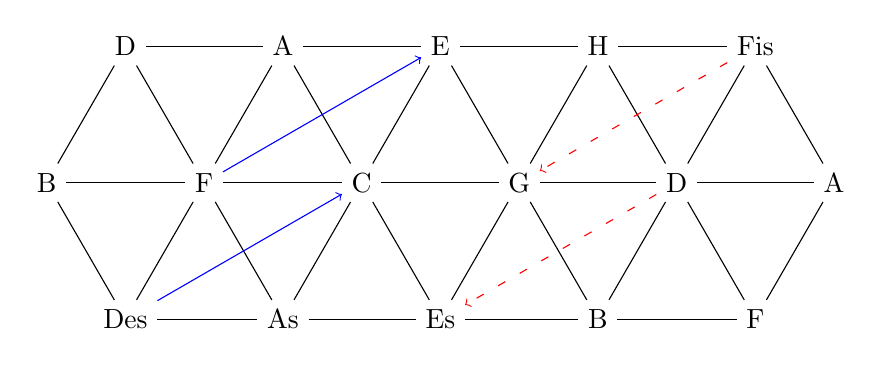
\begin{tikzpicture}[scale=2]
  \tikzset{note/.style={shape=circle,text centered,draw}};
  \node (T) at (0,0){C};
  \node (D) at (1,0){G};
  \node (S) at (-1,0){F};
  \node (M) at (60:1){E};
  \node (m) at (-60:1){Es};
  \node (SM) at ($(S)+(M)$) {A};
  \node (Sm) at ($(S)+(m)$) {As};
  \node (DD) at ($(D)+(D)$) {D};
  \node (DM) at ($(D)+(M)$){H};
  \node (Dm) at ($(D)+(m)$){B};
  \node (SS) at ($(S)+(S)$) {B};
  \node (SSM) at ($(SS)+(M)$) {D};
  \node (SSm) at ($(SS)+(m)$) {Des};
  \node (DDD) at ($(DD)+(D)$) {A};
  \node (DDM) at ($(DD)+(M)$){Fis};
  \node (DDm) at ($(DD)+(m)$){F};
  \draw (SS) -- (S) -- (T) -- (D) -- (DD) -- (DDD);
  \draw (SSM) -- (SM) -- (M) -- (DM) -- (DDM);
  \draw (SSm) -- (Sm) -- (m) -- (Dm) -- (DDm);
  \draw (SS)--(SSM)--(S)--(SM)--(T)--(M)--(D)--(DM)--(DD)--(DDM)--(DDD);
  \draw (SS)--(SSm)--(S)--(Sm)--(T)--(m)--(D)--(Dm)--(DD)--(DDm)--(DDD);
  \draw[red,loosely dashed,font=\tiny,arrows={->}] (DDM) -- (D);
  \draw[red,loosely dashed,font=\tiny,arrows={->}] (DD) -- (m);
  %\draw[red,arrows={->}] (D) to[bend left] (T);
  \draw[blue,font=\tiny,arrows={->}] (SSm) -- (T);
  \draw[blue,font=\tiny,arrows={->}] (S) -- (M);
  %\draw[blue,arrows={->}] (S) to[bend left] (T);
\end{tikzpicture}
\end{document}
